%% Copyright (C) 2010, 2011, Gostai S.A.S.
%%
%% This software is provided "as is" without warranty of any kind,
%% either expressed or implied, including but not limited to the
%% implied warranties of fitness for a particular purpose.
%%
%% See the LICENSE file for more information.

\documentclass[openright,twoside,11pt]{book}
%  \usepackage[svgnames]{xcolor}  \usepackage{experiment}
  \usepackage{gostai-documentation}
  \usepackage{config}
  \usepackage[draft]{showlabels}
  \usepackage{lipsum}  % to provide "filler" text

% \grammar{RANGE}
% ---------------
% For instance
%
%   \grammar{arithmetic-exp}
%   \grammar{class-exp, lvalue-end, block-exp}
%   \grammar{}
%
% Beware that the RANGE items must be in order in the file: the file is
% *not* read several times.
%
% It may seem that having a rangesuffix is useless, but actually without
% it markups such as "catch" and "catchall" both match "catch".  Luckily,
% we can use \^^M which, in TeX parlance, means end-of-line.
\newcommand{\grammar}[1]{%
  \bnfPre%
  \lstinputlisting[style=UrbiSDKEnv,
                   backgroundcolor=\color{bnf},
                   language=bnf,
                   morecomment={[is]{\#:}{\^^M}},
                   includerangemarker=false,
                   rangeprefix={\#:},rangesuffix={\^^M},
                   linerange={#1}]
          {tables/urbiscript.bnf}%
  \bnfPost%
}


\title{Urbi Documentation Sandbox}
\subtitle{Version \VcsDescription}
\author{Gostai}

\begin{document}

\maketitle

This document is meant to be used to toy with \LaTeX{}.

\tableofcontents
\part{First Part}

\chapter{First Chapter}

This is the first chapter.

\grammar{class-exp, lvalue-end, block-exp}

\begin{verbatim}
for (var i: 10)
  echo(i);
\end{verbatim}

\begin{urbiunchecked}
'if' + 'else' + 'bitand';
'if'+'else'+'bitand';
'if'.'else'.'bitand';
.'else';

x xor_eq a;

a.'bitand'(b);
a' "foo";
a'' "foo";
a''' "foo";
"else";

"foo";
[00048238] "foo"
\end{urbiunchecked}

\grammar{}

\begin{verbatim}
for (var i: 10)
  echo(i);
\end{verbatim}

\begin{verbatim}[language=gdb]
(gdb) urbi break input.u:2 Lobby_0x7ffff7f03208.foo(["2" => 2])
UBreakpoint 1:
        Location: input.u:2
        Lobby_0x7ffff7f03208.foo(["2" => 2])
(gdb) c
Continuing.

//#push 1 "input.u"
function foo (x) { backtrace }|;
for(var i: [1, 2, 3]) foo([i.asString => i]);

[00219506:backtrace] foo (input.u:2.23-44)
[00219506:backtrace] each (input.u:2.12-44)
UBreakpoint 1: [input.u:2.23-45] Lobby_0x7ffff7f03208.foo(["2" => 2])
Inside Job 0x6a2f70
(gdb) urbi stack
#12 [input.u:1.20-29] Lobby_0x7ffff7f03208.backtrace()
#16 [input.u:1.20-29] Call backtrace
#55 [input.u:2.1-40] Stmt
(gdb) #% comment
\end{verbatim}

\noindent
\begin{minipage}[t]{.48\linewidth}
\begin{urbiscript}[xrightmargin=0mm,xleftmargin=0mm]
class ImmutableCounter : Counter
{
  function '+='(var n) { this + n };
  function '-='(var n) { this - n };
}|;

var ic1 = ImmutableCounter.new(0);
[00010566] 0 @ 0x100354b70
var ic2 = ic1;
[00010574] 0 @ 0x100354b70

ic1 += 1;
[00010588] 1 @ 0x10875bee0

// ic1 points to a new object.
ic1;
[00010592] 1 @ 0x10875bee0
// ic2 still points to its original value.
ic2;
[00010594] 0 @ 0x100354b70
\end{urbiscript}
\end{minipage}
\hfill
\begin{minipage}[t]{.48\linewidth}
\begin{urbiscript}[xrightmargin=0mm,xleftmargin=0mm]
class MutableCounter : Counter
{
  function '+='(var n) { count += n | this };
  function '-='(var n) { count -= n | this };
}|;

var mc1 = MutableCounter.new(0);
[00029902] 0 @ 0x100364e00
var mc2 = mc1;
[00029911] 0 @ 0x100364e00

mc1 += 1;
[00029925] 1 @ 0x100364e00

// mc1 points to the same, updated, object.
mc1;
[00029930] 1 @ 0x100364e00
// mc2 too.
mc2;
[00029936] 1 @ 0x100364e00
\end{urbiscript}
\end{minipage}


\begin{urbiscript}[multicols=2]
class ImmutableCounter : Counter
{
  function '+='(var n) { this + n };
  function '-='(var n) { this - n };
}|;

var ic1 = ImmutableCounter.new(0);
[00010566] 0 @ 0x100354b70
var ic2 = ic1;
[00010574] 0 @ 0x100354b70

ic1 += 1;
[00010588] 1 @ 0x10875bee0

// ic1 points to a new object.
ic1;
[00010592] 1 @ 0x10875bee0
// ic2 still points to its original value.
ic2;
[00010594] 0 @ 0x100354b70
class MutableCounter : Counter
{
  function '+='(var n) { count += n | this };
  function '-='(var n) { count -= n | this };
}|;

var mc1 = MutableCounter.new(0);
[00029902] 0 @ 0x100364e00
var mc2 = mc1;
[00029911] 0 @ 0x100364e00

mc1 += 1;
[00029925] 1 @ 0x100364e00

// mc1 points to the same, updated, object.
mc1;
[00029930] 1 @ 0x100364e00
// mc2 too.
mc2;
[00029936] 1 @ 0x100364e00
\end{urbiscript}


\begin{urbiassert}
1+2 == 3;
\end{urbiassert}

% \release{Release}{Date}
% -----------------------
\newcommand{\release}[2]{%
  \ifx\ifHtml\undefined%
    Released on #2.
    \marginpar{%
      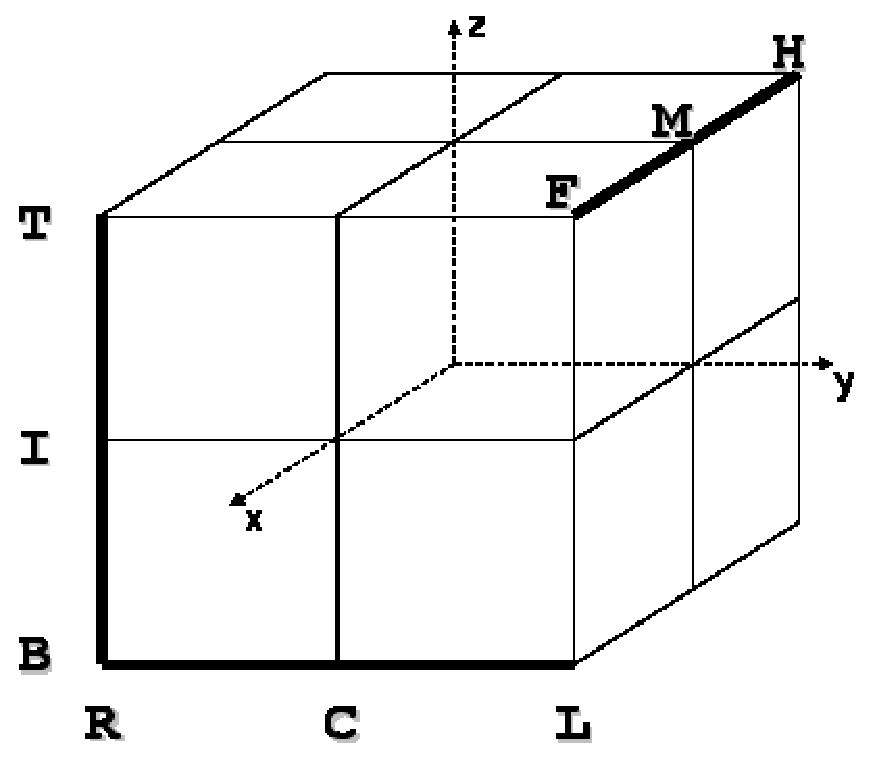
\includegraphics[width=\marginparwidth]{figs/urbi-sdk/#1/cube}

      #2.
    }%
  \else
    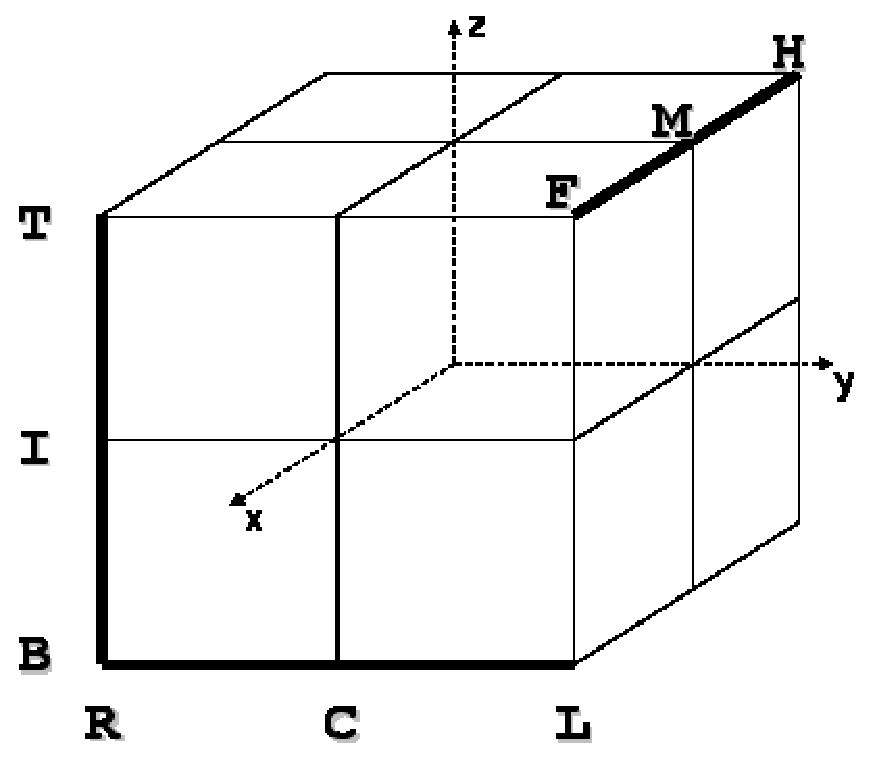
\includegraphics[width=.2\textwidth]{figs/urbi-sdk/#1/cube},
    released on #2.
  \fi%
}

\section{\usdk 2.5}
\release{2.5}{2010-11-xx}

\subsection{New Features}
\begin{itemize}
\item More types of empty statements are warned about.  For instance \urbi
  used to accept silently \lstinline|if (foo);|.  It now warns about the empty
  body, and recommends writing \lstinline|if (foo) {};|.
\end{itemize}

\section{\usdk 2.4}
\release{2.4}{2010-11-xx}

\subsection{New Features}
\begin{itemize}
\item More types of empty statements are warned about.  For instance \urbi
  used to accept silently \lstinline|if (foo);|.  It now warns about the empty
  body, and recommends writing \lstinline|if (foo) {};|.
\end{itemize}

\section{\usdk 2.3}
\release{2.3}{2010-11-xx}

\subsection{New Features}
\begin{itemize}
\item More types of empty statements are warned about.  For instance \urbi
  used to accept silently \lstinline|if (foo);|.  It now warns about the empty
  body, and recommends writing \lstinline|if (foo) {};|.
\end{itemize}


\sectionObject{Bar}

\begin{urbiscriptapi}
\item[bar] This is Bar.bar.
\item[foo](<x>) This is Bar.foo with arguments.
\item[set](<key>, <value>) Map \var{key} to \var{value} and return \this so
  that invocations to \lstinline|set| can be chained.  The possibly existing
  previous mapping is overridden.
\item \lstinline|I do it myself|
\item beware (not to catch the first word)
\item|slot[foo][bar]| a slot
\item|fun[foo][bar]|(<var>) a function
\end{urbiscriptapi}

\sectionObject{Foo}

\begin{urbiscriptapi}
\item[bar] This is Foo.bar.
\item[foo] This is Foo.foo.
\end{urbiscriptapi}

\section{Second Section}

\begin{urbiunchecked}[escapeinside=<>]
#<Été>;
[00048238:error] !!! invalid character: `#'
[00048239:error] !!! invalid character: `\xc3'
[00048239:error] !!! invalid character: `\x89'
[00048239:error] !!! invalid character: `\xc3'
[00048239:error] !!! invalid character: `\xa9'
\end{urbiunchecked}

\chapter{Second Chapter}

This is the second chapter.

\urbitrajectory{smooth}

\urbitrajectory{accel}

\begin{urbiscriptapi}
\item[count] Return the count.
\item[launch]
  Fire \this.
\item \lstinline|launch|~\\
  Fire \this.
\end{urbiscriptapi}

\let\sectionOrig\section
\renewcommand{\section}[1]{\clearpage\sectionObject{#1}}
\section{Pair}

A \dfn{pair} is a container storing two objects, similar in spirit to
\lstinline|std::pair| in \Cxx.

\subsection{Prototype}
\begin{itemize}
\item \refObject{Object}
\end{itemize}

\subsection{Construction}

A \dfn{Pair} is contructed with one or two arguments. In case on one
argument used, the constructor uses it twice.

\begin{urbiscript}
Pair.new(1, 2);
[00000001] (1, 2)
Pair.new(3);
[00000002] (3, 3)
\end{urbiscript}

\subsection{Methods}
\begin{itemize}
\item \lstinline|asString|\\
  Generate the string \samp{(\var{first}, \var{second})} using
  \code{asPrintable} to convert members to strings.

\item \lstinline|first|\\
  Return the first member of the pair.
\begin{urbiscript}[firstnumber=last]
assert(Pair.new(1, 2).first == 1);
\end{urbiscript}

\item \lstinline|second|\\
  Return the second member of the pair.
\begin{urbiscript}[firstnumber=last]
assert(Pair.new(1, 2).second == 2);
\end{urbiscript}

\item \lstinline|'[]'(\var{index})|\\
  Return the \var{index}-th element.  \var{index} must be 0 or 1.
\begin{urbiscript}[firstnumber=last]
assert(Pair[0] === Pair.first);
assert(Pair[1] === Pair.second);
\end{urbiscript}

\item \lstinline|'[]='(\var{index}, \var{value})|\\
  Set (and return) the \var{index}-th element to \var{value}.
  \var{index} must be 0 or 1.

\item \lstinline|'<'(\var{other})|\\
  Lexicographic comparison between two pairs.
\begin{urbiscript}[firstnumber=last]
assert(Pair.new(0, 0) < Pair.new(0, 1));
assert(Pair.new(0, 0) < Pair.new(1, 0));
assert(Pair.new(0, 1) < Pair.new(1, 0));
\end{urbiscript}

\item \lstinline|'=='(\var{other})|\\
  Whether \lstinline|this| and \lstinline|other| have the same
  contents (equality-wise).
\begin{urbiscript}[firstnumber=last]
assert(Pair.new(1, 2) == Pair.new(1, 2));
assert(!(Pair.new(1, 1) == Pair.new(2, 2)));
\end{urbiscript}
\end{itemize}



%%% Local Variables:
%%% mode: latex
%%% TeX-master: "../urbi-sdk"
%%% End:

\let\section\sectionOrig


\part{Second Part}
\label{sec:second}
This is the second part.

\chapter{Chapter II.1}

You want to use \refSlot[Foo]{foo}, and possibly \refSlot[Bar]{foo}.
\settocbibname{\label{sec:bib}The Bibliography}
\setindexname{\label{sec:index}The Index}
\bibliographystyle{plain}
\bibliography{comp.lang.urbi}
\nocite{*}

\chapterIndex
\end{document}

%%% Local Variables:
%%% mode: latex
%%% coding: utf-8
%%% TeX-master: t
%%% ispell-dictionary: "american"
%%% ispell-personal-dictionary: "urbi.dict"
%%% fill-column: 76
%%% End:
